\comment{
J'enleve cette partie car nous nous sommes apercu que les boucles sans
controle du nombre d'iteration sont perverses. A voir avec les
conditions.

\subsection{Spirales et carr\'es} 
En reprenant les spirales des le\c cons pr\'ec\'edentes essayez de
g\'en\'erer les figures suivantes. Pour les obtenir nous avons cr\'e\'e
une nouvelle m\'ethode qui dessine un carr\'e de 10 pixels de
c\^ot\'e.

\begin{figure}[!htbp]
\centerline{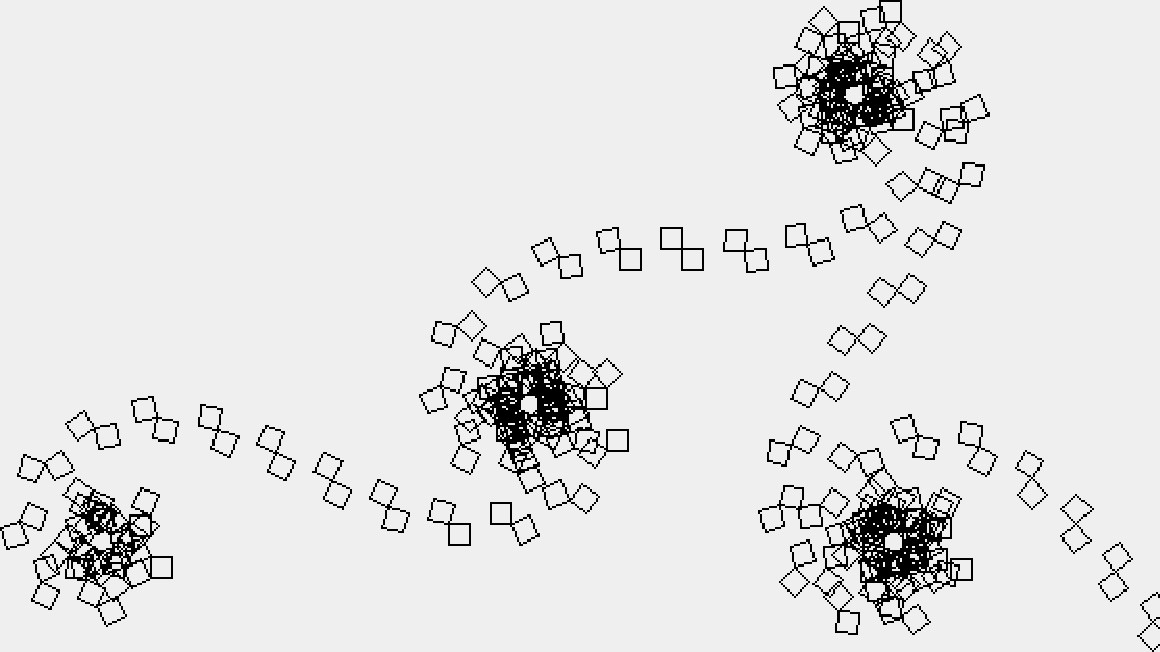
\includegraphics[width=7.5cm]{c7spiralcarre}}
\caption{Composons un labyrinthe et des carr\'es.}
\label{c7spiralcarre}
\end{figure}

\begin{ncscript}{Spirales carr\'eifi\'ees}
| caro angle |
caro := Turtle new.
angle := 119.
1200 timesRepeat: [caro square10.
                  caro turnLeft: angle.
                  caro go: 30.
                  angle := angle + 7]
\end{ncscript}
}
